\chapter{LLM Application Architecture Patterns}
\label{ch:app-architecture}

\begin{quote}
\itshape
``Architecture is the decisions you wish you could get right early.''\\
--- Ralph Johnson
\end{quote}

\vspace{0.5cm}

\noindent
Building a prototype with an LLM takes hours. Building a production system takes months. The gap between the two is almost entirely architectural: how you manage prompts, assemble context, route requests, validate outputs, handle failures, and maintain quality at scale. This chapter describes the architecture patterns that have emerged from the first wave of production LLM applications.

\section{The Canonical LLM Application Stack}

Every production LLM application, regardless of use case, shares a common set of architectural concerns. Figure~\ref{fig:canonical-stack} shows the canonical stack that we see across successful deployments.

\begin{figure}[htbp]
\centering
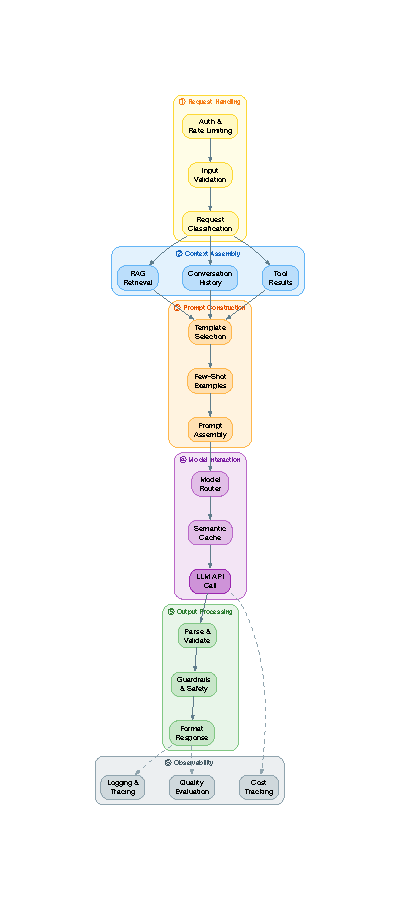
\includegraphics[width=\textwidth]{diagrams/compiled/ch05/canonical-stack.pdf}
\caption{The canonical LLM application stack}
\label{fig:canonical-stack}
\end{figure}

The stack has six layers, each with its own design challenges:

\begin{enumerate}[leftmargin=*]
    \item \textbf{Request handling}: Input validation, rate limiting, authentication
    \item \textbf{Context assembly}: Retrieving relevant information (RAG, tool calls, conversation history)
    \item \textbf{Prompt construction}: Templating, few-shot example selection, instruction formatting
    \item \textbf{Model interaction}: Model selection, routing, retry logic, streaming
    \item \textbf{Output processing}: Parsing, validation, guardrails, formatting
    \item \textbf{Observability}: Logging, tracing, evaluation, cost tracking
\end{enumerate}

\section{Prompt Engineering as Software Engineering}

Prompts are the new source code. In a traditional application, business logic lives in functions and classes. In an LLM application, a significant portion of the business logic lives in prompts. This means prompts deserve the same engineering rigor as code: versioning, testing, review, and CI/CD.

\subsection{The Prompt Lifecycle}

Production prompt management follows the same lifecycle as any software artifact: authoring, testing, review, deployment, and monitoring. The key difference is that a prompt change can silently degrade quality without any compilation error or test failure.

\begin{figure}[htbp]
\centering
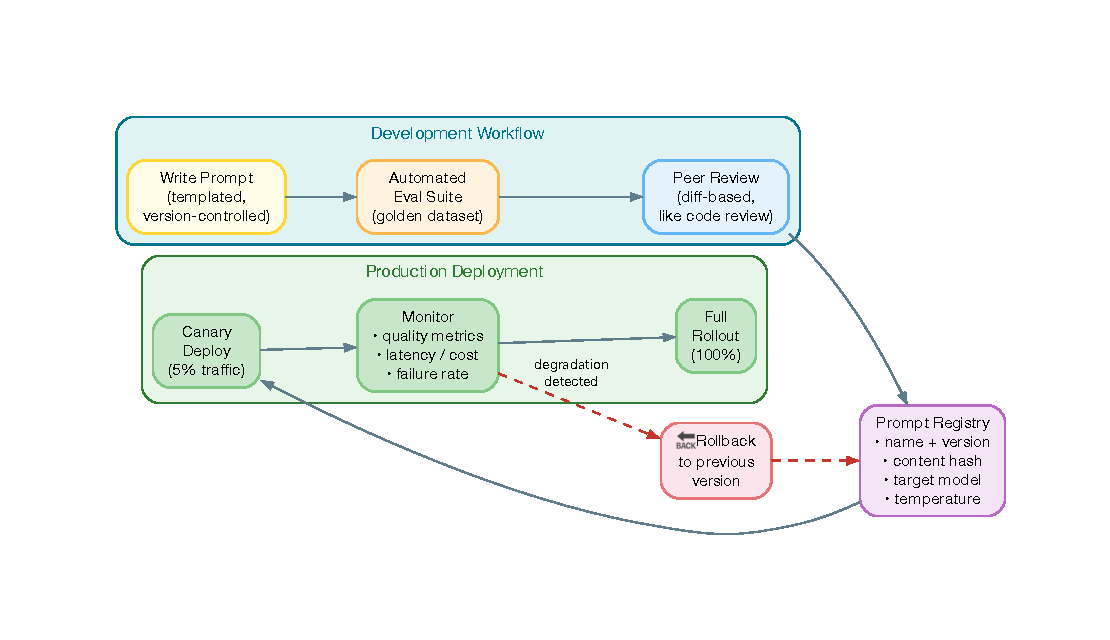
\includegraphics[width=\textwidth]{diagrams/compiled/ch05/prompt-lifecycle.pdf}
\caption{The prompt lifecycle: prompts follow the same CI/CD discipline as code, including canary deployments and automated rollback}
\label{fig:prompt-lifecycle}
\end{figure}

A production prompt management system needs five capabilities:

\begin{enumerate}[leftmargin=*]
    \item \textbf{Version control}: Every prompt is identified by a name, version, and content hash. Changes are tracked in Git alongside application code, enabling meaningful diffs and blame.
    \item \textbf{Model binding}: Prompts are written \emph{for} a specific model. A prompt optimized for GPT-5.5 will often perform poorly on Claude Opus 4.8 and vice versa. The registry tracks which model each prompt targets.
    \item \textbf{Automated evaluation}: Before deployment, every prompt change runs against a golden dataset of (input, expected\_output) pairs. Regressions block the deploy.
    \item \textbf{Canary deployment}: New prompt versions initially serve 5--10\% of traffic while quality metrics are monitored. Only after passing a confidence threshold does the new version roll out fully.
    \item \textbf{Instant rollback}: When a prompt change causes quality degradation in production, the system rolls back to the previous version within seconds---no code deploy needed.
\end{enumerate}

Teams that treat prompts as configuration rather than code invariably regret it. At scale, a single poorly-phrased system prompt can affect millions of requests before anyone notices.


\subsection{Structured Outputs and Function Calling}

One of the most important patterns for production LLM applications is constraining the model's output to a specific structure. This eliminates the need for fragile output parsing and makes LLM calls behave more like traditional API calls.

\begin{lstlisting}[language=Python, caption={Structured output with Pydantic validation}]
from pydantic import BaseModel, Field
from enum import Enum

class Sentiment(str, Enum):
    POSITIVE = "positive"
    NEGATIVE = "negative"
    NEUTRAL = "neutral"

class SentimentAnalysis(BaseModel):
    """Structured output for sentiment analysis."""
    sentiment: Sentiment
    confidence: float = Field(ge=0.0, le=1.0)
    key_phrases: list[str] = Field(max_length=5)
    reasoning: str

def analyze_sentiment(text: str) -> SentimentAnalysis:
    """Analyze sentiment with guaranteed structured output."""
    response = client.chat.completions.create(
        model="gpt-5.5",
        messages=[
            {"role": "system", "content": "Analyze sentiment."},
            {"role": "user", "content": text},
        ],
        response_format={
            "type": "json_schema",
            "json_schema": {
                "name": "sentiment_analysis",
                "schema": SentimentAnalysis.model_json_schema(),
            }
        },
    )
    return SentimentAnalysis.model_validate_json(
        response.choices[0].message.content
    )
\end{lstlisting}

\section{Retrieval-Augmented Generation (RAG)}
\label{sec:rag}

RAG~\cite{lewis2020rag} is the most important architecture pattern for LLM applications that need access to private, recent, or specialized knowledge. The core idea is simple: instead of relying solely on the model's parametric knowledge (what it learned during pre-training), you \emph{retrieve} relevant documents from an external knowledge base and include them in the prompt context.

\subsection{The RAG Pipeline}

\begin{figure}[htbp]
\centering
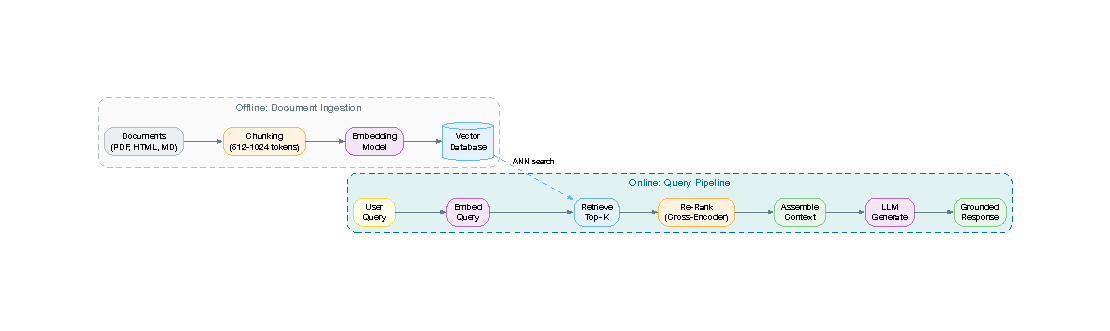
\includegraphics[width=\textwidth]{diagrams/compiled/ch05/rag-pipeline.pdf}
\caption{The RAG pipeline: from user query to grounded response}
\label{fig:rag-pipeline}
\end{figure}

A production RAG pipeline has five stages:

\textbf{1. Document ingestion and chunking.} Documents are split into chunks of manageable size (typically 256--1024 tokens). The chunking strategy you choose has a surprisingly large impact on retrieval quality. Figure~\ref{fig:chunking-strategies} compares the three dominant approaches.

\begin{figure}[htbp]
\centering
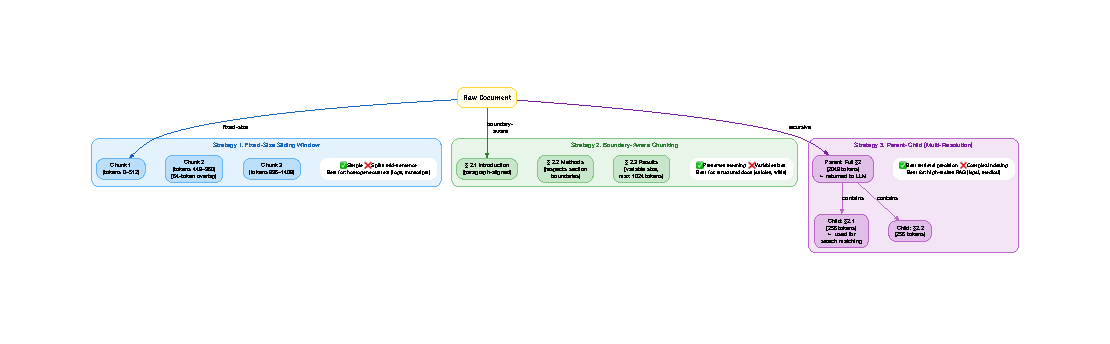
\includegraphics[width=\textwidth]{diagrams/compiled/ch05/chunking-strategies.pdf}
\caption{Three chunking strategies compared: fixed-size sliding window (simple but splits context), boundary-aware (preserves semantics), and parent-child multi-resolution (best precision, most complex)}
\label{fig:chunking-strategies}
\end{figure}

The choice depends on your document types and retrieval precision requirements:

\begin{itemize}[leftmargin=*]
    \item \textbf{Fixed-size}: Best for homogeneous text (logs, transcripts). Simple to implement, but can split mid-sentence.
    \item \textbf{Boundary-aware}: Best for structured content (articles, documentation). Respects paragraph and section boundaries.
    \item \textbf{Parent-child}: Best for high-stakes applications (legal, medical). Small chunks are used for search matching, but the full parent section is returned to the LLM for context.
\end{itemize}

\textbf{2. Embedding.} Each chunk is converted to a dense vector using an embedding model. As of mid-2026, the leading options include OpenAI's embedding models, Google's Gecko, and open-source models like BGE-M3 and E5-Mistral.

\textbf{3. Indexing.} Embeddings are stored in a vector database (Pinecone, Weaviate, Qdrant, pgvector, Milvus) for efficient similarity search.

\textbf{4. Retrieval.} Given a user query, the system retrieves the most relevant chunks. The best practice is \emph{hybrid search}---combining dense and sparse retrieval---followed by \emph{re-ranking}. We cover this in detail below.

\textbf{5. Generation.} The retrieved chunks are included in the prompt context, and the LLM generates a response grounded in the retrieved information.


\subsection{Hybrid Search: Dense + Sparse}

Neither dense retrieval nor sparse retrieval alone provides optimal results. Dense retrieval excels at semantic matching (understanding that ``car'' and ``automobile'' are related) but can miss exact keyword matches. Sparse retrieval (BM25) excels at exact matching but misses semantic relationships.
\begin{figure}[htbp]
\centering
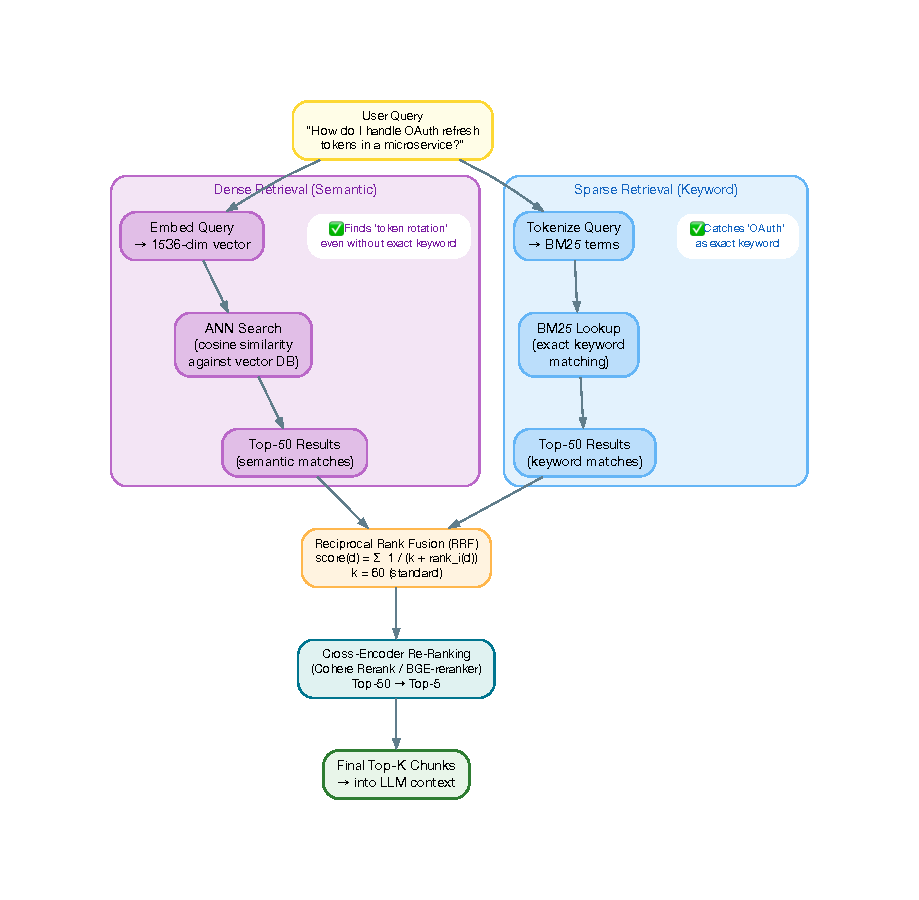
\includegraphics[width=\textwidth]{diagrams/compiled/ch05/hybrid-search.pdf}
\caption{Hybrid search architecture: dense (semantic) and sparse (keyword) retrieval paths are fused via Reciprocal Rank Fusion, then a cross-encoder re-ranks the top candidates}
\label{fig:hybrid-search}
\end{figure}

The key design decisions in a hybrid search system:

\begin{itemize}[leftmargin=*]
    \item \textbf{Dense-to-sparse weight ratio}: Start with 0.7 dense / 0.3 sparse and tune from there. Semantic-heavy queries (``how do I handle token rotation?'') benefit from higher dense weight; keyword-heavy queries (``OAuth RFC 6749'') benefit from higher sparse weight.
    \item \textbf{Fusion method}: Reciprocal Rank Fusion (RRF) is the industry standard. It computes $\text{score}(d) = \sum_i \frac{1}{k + \text{rank}_i(d)}$ where $k = 60$ is the standard smoothing constant. RRF is preferred over score-based fusion because it is robust to score distribution differences between retrieval methods.
    \item \textbf{Re-ranking}: A cross-encoder re-ranker examines each (query, document) pair jointly and produces a relevance score. This is far more accurate than the initial bi-encoder retrieval but too expensive to run on the full corpus---hence the two-stage architecture.
    \item \textbf{Query expansion}: For complex queries, use the LLM to generate 3--5 reformulations (e.g., ``What are the OAuth refresh token best practices for distributed systems?'' $\to$ ``token rotation microservice,'' ``OAuth 2.0 refresh grant flow''). Run each reformulation through retrieval and deduplicate results.
\end{itemize}

\section{Multi-Model Architectures}

Production applications increasingly use multiple models for different tasks, routing requests to the most appropriate model based on complexity, cost, and latency requirements. Figure~\ref{fig:model-routing} shows a typical three-tier routing architecture with semantic caching and quality-based fallback.

\begin{figure}[htbp]
\centering
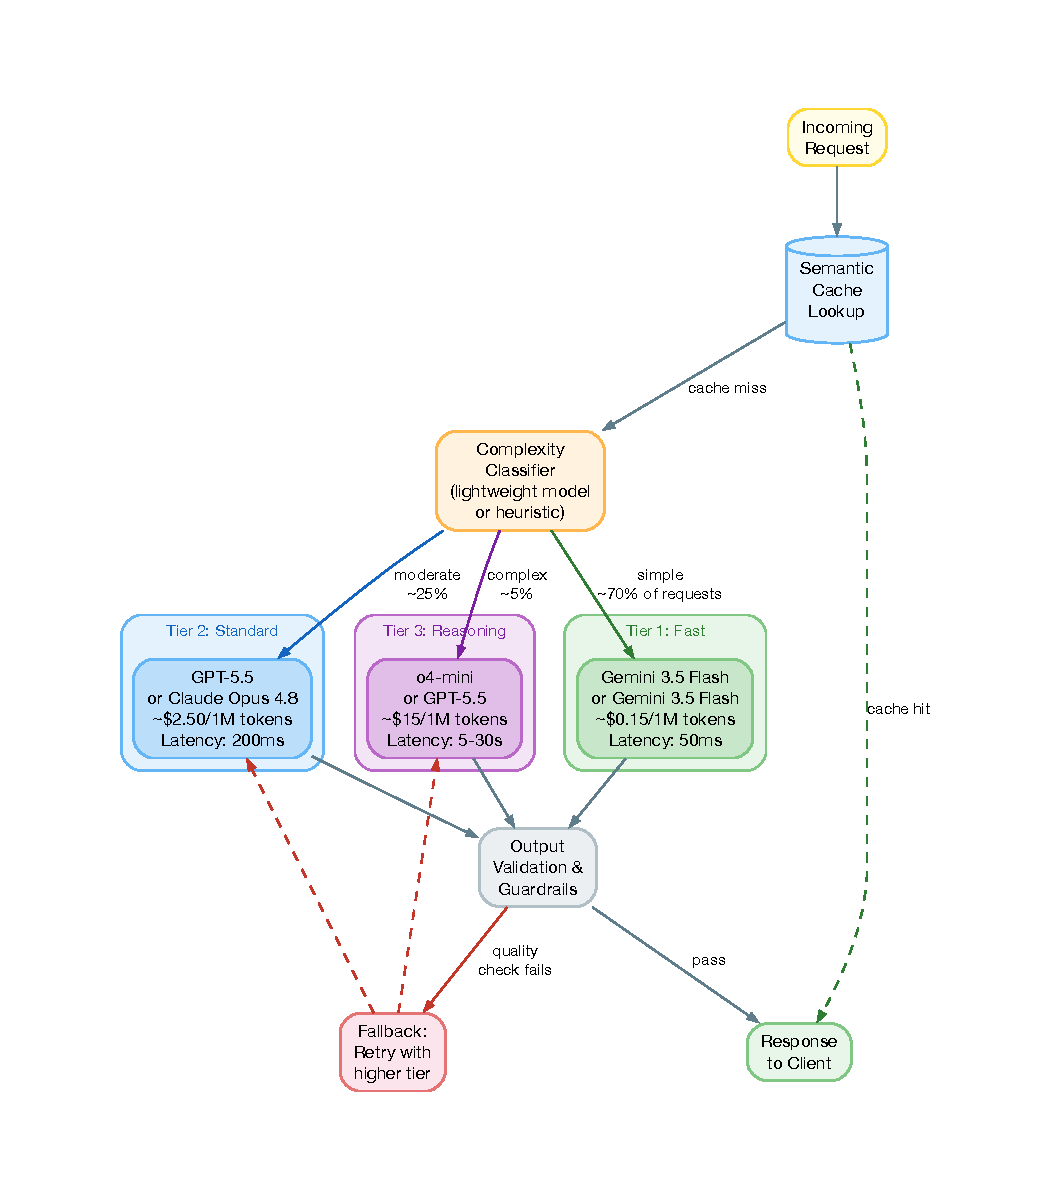
\includegraphics[width=\textwidth]{diagrams/compiled/ch05/model-routing.pdf}
\caption{Multi-model routing: semantic cache $\to$ complexity classifier $\to$ three model tiers with quality-based fallback}
\label{fig:model-routing}
\end{figure}

\subsection{Model Routing Design}
\label{sec:model-routing}

The economics of model routing are compelling. In a typical production workload:

\begin{itemize}[leftmargin=*]
    \item \textbf{$\sim$70\% of requests are simple}: Lookups, reformatting, classification, short answers. These can be handled by fast, inexpensive models like Gemini 3.5 Flash at \$0.15 per million tokens.
    \item \textbf{$\sim$25\% are moderate}: Multi-step reasoning, summarization, code generation. Models like GPT-5.5 or Claude Opus 4.8 handle these well at \$2--5 per million tokens.
    \item \textbf{$\sim$5\% are complex}: Deep analysis, long-context reasoning, novel problem solving. These require premium reasoning models at \$10--15 per million tokens.
\end{itemize}

Without routing, you pay premium prices for every request. With routing, you can reduce average cost by 5--10x while maintaining quality. The classifier itself can be a small fine-tuned model or even a rule-based system---it doesn't need to be perfect, just good enough to route the obvious cases correctly.

A critical design decision: \textbf{quality-based fallback}. When the output from a fast model fails validation (wrong format, low confidence, factual inconsistency), the system automatically retries with a higher-tier model. This lets you aggressively route to cheap models knowing that failures will be caught and escalated.


\begin{keytakeaway}
The architecture of an LLM application is where engineering discipline matters most. A well-designed prompt management system, a robust RAG pipeline, and intelligent model routing can make the difference between a demo that impresses and a product that works. Invest in these infrastructure components early---they are far harder to retrofit than to build from the start.
\end{keytakeaway}


\subsection{Native Prompt Caching}

One of the most impactful---and underappreciated---optimizations in modern LLM APIs is \textbf{native prompt caching} (also called prefix caching). All major providers now cache the KV-cache states for prompt prefixes that remain stable across requests. If your system prompt, few-shot examples, and tool definitions total 5,000 tokens, and only the user query varies, you pay full price on the first request---but subsequent requests with the same prefix receive a 50--90\% discount on input tokens and 60--80\% lower latency (because the cached KV states skip the prefill phase entirely).

This fundamentally changes the architecture of prompt systems:

\begin{itemize}[leftmargin=*]
    \item \textbf{Long system prompts are now cheap}: Previously, engineers compressed system prompts to save costs. With prefix caching, you should \emph{invest} in rich, detailed system prompts because the marginal cost of additional prefix tokens approaches zero.
    \item \textbf{Prompt structure matters}: Place \emph{all} stable content (system prompt, few-shot examples, tool definitions, reference documents) at the \emph{beginning} of the prompt. Place variable content (user query) at the \emph{end}. The cache matches by prefix---any change in the middle invalidates everything after it.
    \item \textbf{Session continuity}: Multi-turn conversations benefit automatically---the growing conversation history is prefix-cached between turns.
    \item \textbf{Impact on cost models}: Combined with model routing and semantic caching, prompt caching can reduce per-request costs by 70--90\% for high-volume applications with stable system prompts.
\end{itemize}

\begin{cautionbox}[Cache Invalidation]
Prompt caches are ephemeral and provider-managed---you have no explicit control over eviction. In practice, caches persist for 5--15 minutes of inactivity. Design your prompt systems with consistent prefix ordering, and monitor cache hit rates through provider dashboards.
\end{cautionbox}
\section{Design Patterns for the Foundation Model Era}
\label{sec:design-patterns}

The Gang of Four gave us a shared vocabulary for object-oriented design. The distributed systems community gave us circuit breakers, sagas, and event sourcing. Now the foundation model era demands its own pattern language: a set of named, reusable solutions to problems that are unique to probabilistic AI systems.

These patterns are not theoretical. They have been extracted from production systems at companies running LLMs at scale, and they address the specific failure modes that make AI systems different from traditional software: non-deterministic outputs, hallucination loops, context window limits, ``Denial of Wallet'' attacks, and the fundamental tension between autonomy and control.

Figure~\ref{fig:design-patterns-catalog} shows the complete catalog organized by category.

\begin{figure}[htbp]
\centering
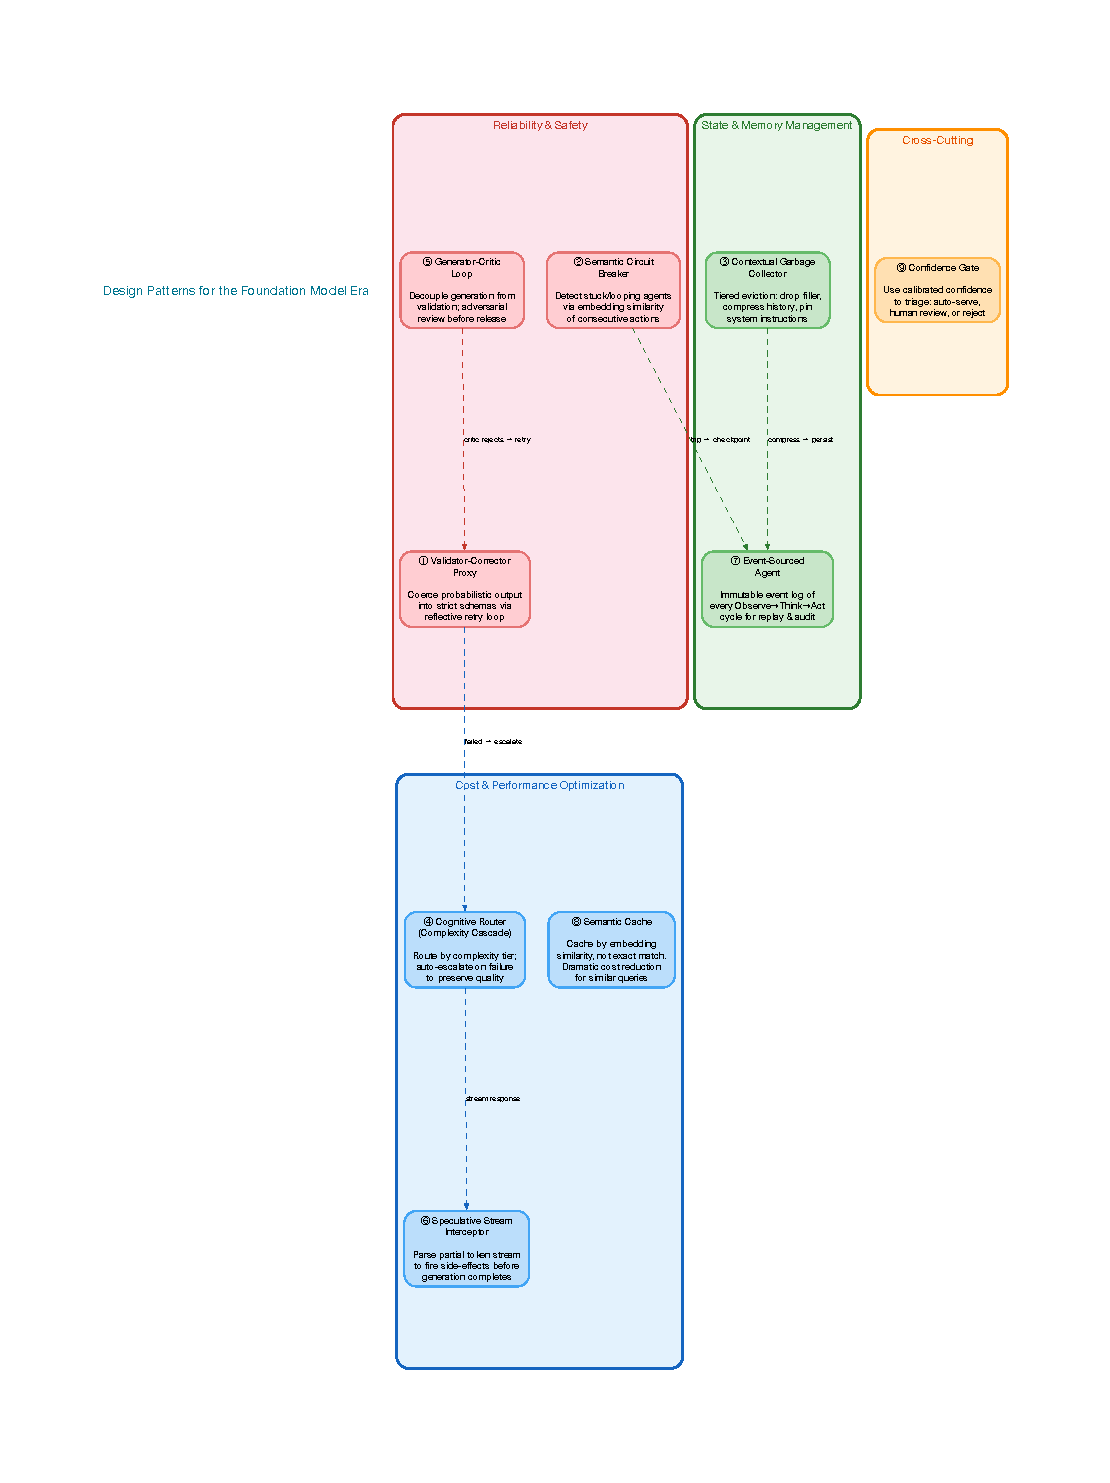
\includegraphics[width=\textwidth]{diagrams/compiled/ch05/design-patterns-catalog.pdf}
\caption{Nine design patterns for the foundation model era, organized by category. Dashed arrows show composition relationships: patterns are designed to work together.}
\label{fig:design-patterns-catalog}
\end{figure}


\subsection{Pattern 1: The Validator-Corrector Proxy}

\textbf{Category}: Reliability \hfill \textbf{Also known as}: Reflective Retry, Self-Healing Parser

\textbf{Intent}: Coerce probabilistic, unstructured text generation into strict, deterministic software contracts without hardcoding edge cases.

\textbf{Motivation}: Traditional software requires strict data schemas---typed arguments, valid JSON, enum values within defined sets. LLMs frequently hallucinate schema properties, omit brackets, wrap JSON in markdown fences, or invent enum values that don't exist. Crashing the application on an unparseable string is unacceptable, but so is shipping malformed data downstream.

\textbf{Mechanism}: Wrap the foundation model in a Proxy layer (Figure~\ref{fig:validator-corrector}). The application never interfaces with the LLM directly. On each call, the Proxy:

\begin{enumerate}[leftmargin=*]
    \item Sends the prompt to the LLM with a structured output schema
    \item Runs the response through a deterministic validator (Pydantic, JSON Schema, regex)
    \item If validation \emph{passes}: returns the typed result to the application
    \item If validation \emph{fails}: catches the exception, appends the \emph{exact error message} to the conversation as a correction prompt (``Your previous output failed validation: \texttt{Expecting property name enclosed in double quotes at line 3}. Fix it and return valid JSON only.''), and re-invokes the LLM
    \item Repeats up to \code{max\_retries} (typically 3), then falls back to a default value or raises to the application
\end{enumerate}

\begin{figure}[htbp]
\centering
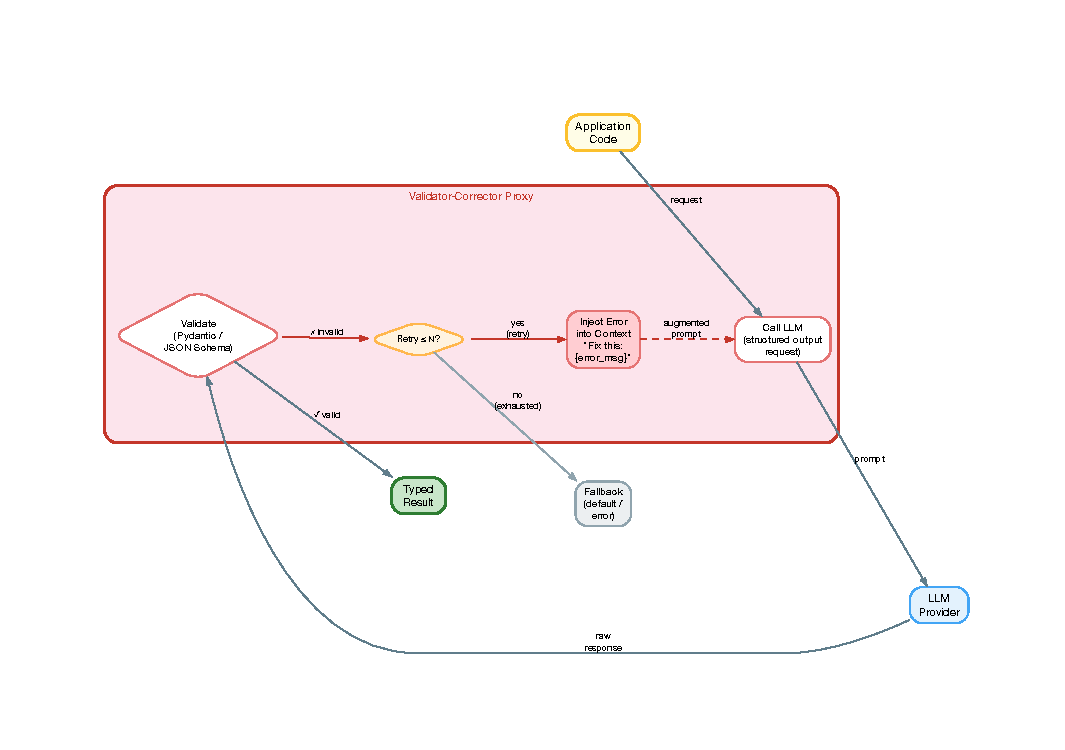
\includegraphics[width=\textwidth]{diagrams/compiled/ch05/pattern-validator-corrector.pdf}
\caption{The Validator-Corrector Proxy: validation failures are injected back into the LLM context for self-correction, bounded by a retry limit to prevent infinite loops.}
\label{fig:validator-corrector}
\end{figure}

\textbf{Trade-offs}: Dramatically increases systemic reliability (many teams report going from 92\% to 99.5\%+ schema compliance) and abstracts AI messiness from the core application. But it multiplies token costs and latency during error states---each retry is a full LLM round-trip. The \code{max\_retries} bound is critical: without it, a structurally incapable model will burn tokens indefinitely.

\textbf{When to use}: Any production LLM call that returns structured data. This pattern is so fundamental that it should be the \emph{default} interface to any LLM.

\begin{tipbox}[Constrained Decoding: The Preferred First Line]
Modern providers offer \textbf{constrained decoding} (OpenAI's strict JSON mode, vLLM's guided decoding via XGrammar/Outlines, Anthropic's tool-use schemas) that forces schema compliance \emph{at the logit level}---the tokenizer can only produce valid JSON matching your schema, with zero retries and zero wasted tokens. When available, constrained decoding is strictly superior to the retry loop described above.

The Validator-Corrector Proxy remains essential as a \textbf{fallback layer} for three scenarios: (1) providers or self-hosted models that don't support constrained decoding, (2) complex multi-field business validations that go beyond JSON schema (e.g., ``field A must be greater than field B''), and (3) semantic validations where the output is structurally valid but factually wrong.

\textbf{The recommended production stack}: Constrained decoding as the primary guarantee, with the Validator-Corrector as a retry layer for edge cases that slip through.
\end{tipbox}


\subsection{Pattern 2: The Semantic Circuit Breaker}

\textbf{Category}: Resilience / Security \hfill \textbf{Also known as}: Hallucination Loop Detector, Budget Guardian

\textbf{Intent}: Prevent autonomous agents from entering infinite hallucination loops, performing destructive actions, or burning API budgets (``Denial of Wallet'').

\textbf{Motivation}: Traditional circuit breakers trip on HTTP 500s or latency spikes. An LLM agent, however, can return perfect HTTP 200s while stubbornly attempting the exact same failed database query 100 times in a row, or rapidly deviating from its core directive. The failure mode is \emph{semantic}, not structural.

\textbf{Mechanism}: A middleware component continuously monitors the ``semantic velocity'' of an agent's reasoning loop (Figure~\ref{fig:circuit-breaker}):

\begin{itemize}[leftmargin=*]
    \item \textbf{Repetition detection}: Compute the vector embedding of consecutive actions. If \code{cosine\_similarity(action[N], action[N-1])} exceeds 0.95 for 3+ consecutive loops, the agent is stuck.
    \item \textbf{Error accumulation}: Track sequential tool-use failures. Three consecutive errors of the same type indicates a systematic problem, not a transient glitch.
    \item \textbf{Budget enforcement}: Monitor cumulative token usage and cost. If a single task exceeds a threshold (e.g., \$5 or 500K tokens), trip the breaker regardless of progress.
    \item \textbf{Drift detection}: Compare the agent's current trajectory against the original goal embedding. If the cosine similarity drops below 0.5, the agent has wandered off-task.
\end{itemize}

\begin{figure}[htbp]
\centering
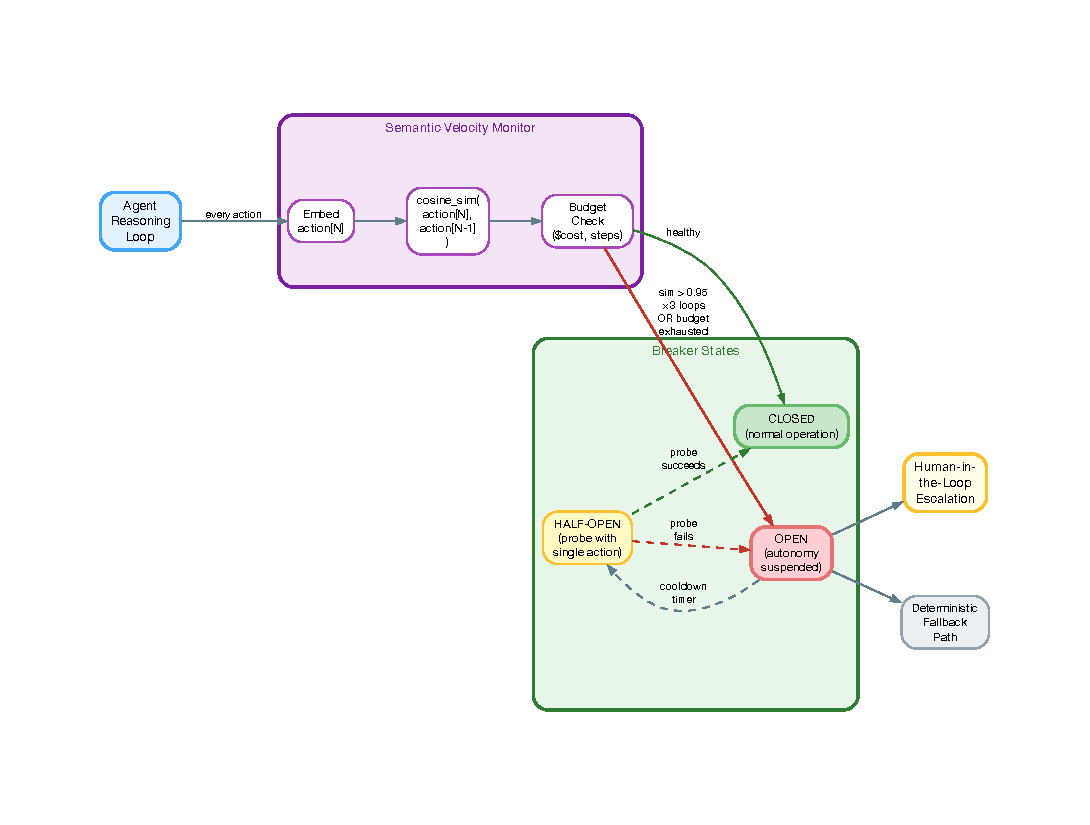
\includegraphics[width=\textwidth]{diagrams/compiled/ch05/pattern-circuit-breaker.pdf}
\caption{The Semantic Circuit Breaker: monitors action embedding similarity and budget to detect stuck loops. Three states mirror the classical circuit breaker pattern: Closed (normal), Open (suspended), Half-Open (probe).}
\label{fig:circuit-breaker}
\end{figure}

When the breaker trips to \emph{Open}, autonomy is suspended: the system either falls back to a deterministic code path or escalates to Human-in-the-Loop (HITL) intervention. After a cooldown period, it transitions to \emph{Half-Open}, allowing a single probe action---if successful, the breaker resets to Closed.

\textbf{Trade-offs}: Prevents runaway costs and destructive loops, but requires careful threshold tuning to avoid false positives on legitimate, highly iterative tasks (e.g., an agent debugging code \emph{should} retry similar actions with small modifications).


\subsection{Pattern 3: The Contextual Garbage Collector}

\textbf{Category}: Memory / State Management \hfill \textbf{Also known as}: Context Window Manager, Tiered Memory Eviction

\textbf{Intent}: Maintain the illusion of infinite memory within finite, computationally expensive context windows without causing agent ``amnesia.''

\textbf{Motivation}: As an agent runs, conversation history and tool outputs bloat the context window. Simple sliding-window (FIFO) truncation is catastrophic: it causes the agent to forget its system instructions or early discoveries. Conversely, passing massive contexts degrades reasoning quality (the ``lost in the middle'' phenomenon) and balloons token costs.

\textbf{Mechanism}: Treat the context window like a tiered memory system. A background daemon monitors active token utilization. When usage reaches $\sim$80\% capacity, the CGC triggers a three-tier eviction policy:

\begin{enumerate}[leftmargin=*]
    \item \textbf{Evict}: Drop conversational filler, intermediate reasoning scratchpads, and verbose tool outputs that have already been acted upon
    \item \textbf{Compress}: Pass older interaction blocks to a fast, cheap model (e.g., Gemini 3.5 Flash) to summarize into dense ``episodic mementos''---a 2000-token conversation becomes a 200-token summary
    \item \textbf{Pin}: Retain the core system instructions, the original user goal, and the compressed summaries as permanent fixtures that never get evicted
\end{enumerate}

\textbf{Trade-offs}: Preserves long-term coherence at significantly lower cost than simply expanding the context window. But granular details from early interactions \emph{will} be lost during compression---if the agent later needs a specific detail from step 3 of a 50-step task, it may not be available. Mitigate by pinning critical intermediate results explicitly.


\subsection{Pattern 4: The Cognitive Router (Complexity Cascade)}

\textbf{Category}: Architectural / Optimization \hfill \textbf{Also known as}: Tiered Model Routing, Smart Gateway

\textbf{Intent}: Optimize the trade-off between operational cost, system latency, and reasoning capability on a per-request basis.

\textbf{Motivation}: Routing every user request to a frontier model (GPT-5.5, Claude Opus 4.8) is economically unviable at scale and introduces unnecessary latency for simple tasks. Conversely, routing everything to a fast, cheap model causes critical failures on complex reasoning tasks.

\textbf{Mechanism}: Implement a dynamic routing layer at the API gateway. Incoming requests are evaluated by an ultra-fast classifier (a fine-tuned micro-model, an embedding similarity check, or keyword-based heuristics) that assigns a complexity tier:

\begin{itemize}[leftmargin=*]
    \item \textbf{Tier 3} (Fast/Cheap): Simple classification, entity extraction, text formatting $\to$ Gemini 3.5 Flash or local model
    \item \textbf{Tier 2} (Standard): Multi-step reasoning, summarization, code generation $\to$ GPT-5.5 or Claude Opus 4.8
    \item \textbf{Tier 1} (Premium): Deep analysis, novel problem solving, critical decisions $\to$ o3 or comparable reasoning model
\end{itemize}

The \emph{Cascade}: if a Tier 3 model fails validation (Pattern 1), expresses low confidence via logprobs, or produces output that fails a quality gate, the router automatically escalates the \emph{exact same prompt} to a higher tier. This lets you aggressively route to cheap models knowing that quality is backstopped.

\textbf{Trade-offs}: Reduces average cost by $5$--$10\times$ for most workloads. But introduces architectural complexity: system prompts must be compatible across model families, and the routing classifier must be maintained alongside the models. We covered the detailed economics in Section~\ref{sec:model-routing} earlier in this chapter.


\subsection{Pattern 5: The Generator-Critic Loop}

\textbf{Category}: Structural / Quality Assurance \hfill \textbf{Also known as}: Dual-Agent Validator, Adversarial Review

\textbf{Intent}: Ensure high-fidelity, aligned outputs by decoupling generation from validation, bypassing the LLM's inherent confirmation bias.

\textbf{Motivation}: Developers often stuff single system prompts with endless negative constraints (``DO NOT do X,'' ``NEVER do Y''), which confuses the model---a phenomenon known as \emph{Negative Prompt Blindness}. Furthermore, a single LLM evaluating its own output naturally suffers from autoregressive confirmation bias: each token is generated to be consistent with the previous tokens, making it structurally difficult for the model to recognize its own errors.

\textbf{Mechanism}: Instantiate two distinct agent roles operating in a loop:

\begin{itemize}[leftmargin=*]
    \item \textbf{Generator}: Operates with a simple, positive prompt focused purely on task completion. No prohibitions, no negative constraints. Its job is to produce the best possible output.
    \item \textbf{Critic}: Operates with a strict, adversarial rubric. It receives the Generator's output and evaluates it against explicit quality criteria. Crucially, the Critic should be a \emph{different model} or at minimum a separate conversation context---it must not share the Generator's confirmation bias.
\end{itemize}

If the Critic rejects the output, it generates structured feedback (not just ``bad''---but specific, actionable corrections). The Generator revises with the Critic's feedback as additional context. The system only releases the output once the Critic approves or a maximum iteration count is reached.

\textbf{Trade-offs}: Multiplies token usage and latency by $2$--$3\times$ per request, but yields near-deterministic quality from a probabilistic system. Use this pattern for high-stakes outputs: customer-facing content, financial calculations, medical summaries, code that will be committed to production.


\subsection{Pattern 6: The Speculative Stream Interceptor}

\textbf{Category}: Concurrency / UX Performance \hfill \textbf{Also known as}: Eager Execution, Partial-Parse Pipeline

\textbf{Intent}: Mask the autoregressive latency of LLMs by executing deterministic side-effects concurrently with token generation.

\textbf{Motivation}: LLMs generate text one token at a time. Waiting for the model to fully generate a JSON payload, then parsing it, then executing the downstream action (database query, API call) creates a blocking, serialized pipeline. The user waits for the model to ``type,'' then waits again for the action to execute.

\textbf{Mechanism}: Implement an Observer pattern that listens to the raw token stream from the model provider in real-time. A partial parser continuously evaluates the incomplete string buffer. As soon as required arguments for a specific action are structurally complete---for example, intercepting \code{\{"query": "SELECT * FROM users"} even before the closing brace arrives---the interceptor spawns a background thread to execute the database call. By the time the model finishes generating its conversational explanation, the data is already fetched and ready to display.

\textbf{Trade-offs}: Dramatically improves perceived performance and time-to-first-useful-byte. But partial JSON parsing is genuinely complex: you need a streaming parser that can detect when a value is ``complete enough'' to act on, handle backtracking when the model changes course, and manage cancellation when the final output invalidates the speculative execution. Libraries like \code{partial-json-parser} help, but edge cases remain. Use this pattern for high-frequency, latency-sensitive applications (conversational agents, real-time coding assistants).


\subsection{Pattern 7: The Event-Sourced Agent}

\textbf{Category}: State Management / Auditing \hfill \textbf{Also known as}: Durable Execution, Checkpoint-Resume Agent

\textbf{Intent}: Capture and externalize the internal reasoning state of an autonomous agent for resumption, auditing, or time-travel debugging.

\textbf{Motivation}: Standard agentic loops run continuously in volatile memory. If an agent executes a 15-step plan and hits an API rate limit on step 14, or if it requires a human to approve an action mid-flight, the ephemeral context is lost. Restarting from scratch is expensive, non-deterministic, and may produce different results.

\textbf{Mechanism}: Apply classical Event Sourcing to the agent's cognition (Figure~\ref{fig:event-sourced}). Every cycle of the agentic loop---Observation $\to$ Thought $\to$ Action---is serialized as an immutable Event object and appended to a durable datastore (Postgres, Redis, or even a structured log file) \emph{before} the next LLM inference call.

\begin{figure}[htbp]
\centering
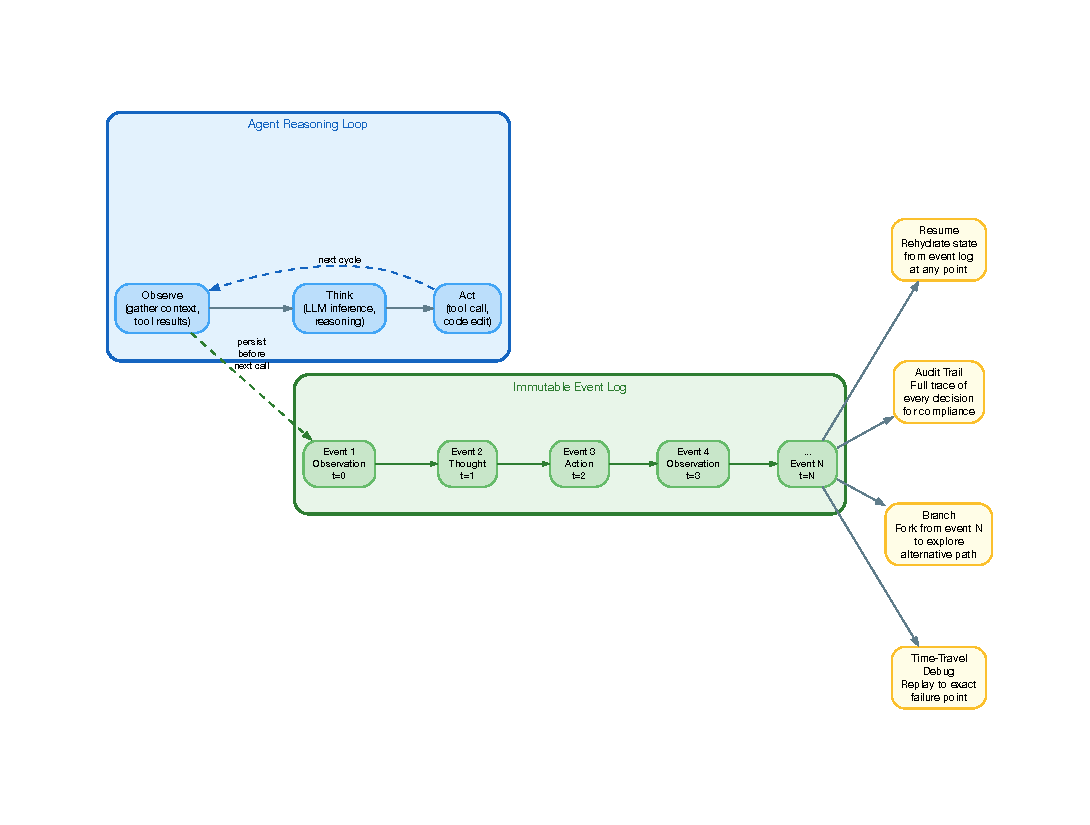
\includegraphics[width=\textwidth]{diagrams/compiled/ch05/pattern-event-sourced.pdf}
\caption{The Event-Sourced Agent: every Observe$\to$Think$\to$Act cycle is persisted as an immutable event, enabling four capabilities: resume from any checkpoint, full audit trail, branch to explore alternatives, and time-travel debugging.}
\label{fig:event-sourced}
\end{figure}

This enables four powerful capabilities:

\begin{itemize}[leftmargin=*]
    \item \textbf{Resume}: If the process is suspended (rate limit, crash, human approval gate), the exact state can be rehydrated by replaying the event log
    \item \textbf{Audit}: Every decision the agent made is recorded with full context. This is essential for regulated industries and for debugging production issues
    \item \textbf{Branch}: Fork the event log at any point to explore alternative paths. ``What if the agent had chosen a different approach at step 7?''
    \item \textbf{Time-travel debugging}: Replay the log to the exact point where the agent went wrong, inspect its context, and understand the failure
\end{itemize}

\textbf{Trade-offs}: Enables HITL pauses, branching logic, and robust retry mechanisms, but requires building a state-management backend rather than relying on simple arrays in local memory. The serialization overhead is negligible compared to LLM inference latency, but the storage cost of full event logs can be significant for long-running agents.


\subsection{Pattern 8: The Semantic Cache}

\textbf{Category}: Cost Optimization \hfill \textbf{Also known as}: Embedding-Based Cache, Approximate Cache

\textbf{Intent}: Avoid redundant LLM calls by serving cached responses for semantically similar (not just identical) queries.

\textbf{Motivation}: Traditional caches use exact-match keys. But users ask the same question in many different ways: ``What's the refund policy?'' and ``How do I get my money back?'' and ``Can I return this for a refund?'' are all the same question. Without semantic caching, each variation triggers a full LLM call.

\textbf{Mechanism}: Embed incoming queries and search the cache for embeddings with cosine similarity above a threshold (typically 0.92--0.97). If a match is found, return the cached response. If not, call the LLM and cache the result with its embedding. Include the prompt version and model ID in the cache key to prevent stale responses after prompt or model updates.

\textbf{Trade-offs}: Can reduce LLM costs by 20--40\% for applications with repetitive query patterns (customer support, documentation Q\&A). But the similarity threshold requires tuning: too low and you serve incorrect cached responses for genuinely different questions; too high and the cache hit rate drops to near-zero. Invalidation is also tricky---when the underlying data changes, cached responses may become stale.


\subsection{Pattern 9: The Confidence Gate}

\textbf{Category}: Cross-Cutting / Human-AI Collaboration \hfill \textbf{Also known as}: Uncertainty Router, Triage Gate

\textbf{Intent}: Use calibrated confidence signals to triage LLM outputs into three paths: auto-serve, human review, or reject.

\textbf{Motivation}: Not all LLM outputs deserve the same level of trust. Some responses the model is highly confident about and are safe to serve directly. Others are uncertain and should be routed to a human reviewer. A few are so low-confidence that they should be rejected outright rather than risk serving a hallucination.

\textbf{Mechanism}: After generating a response, compute a confidence signal from one or more sources: logprobs (token-level probability), self-consistency (generate $N$ responses and measure agreement), or a separate calibration model. Route based on thresholds:

\begin{itemize}[leftmargin=*]
    \item \textbf{High confidence} ($>$ 0.9): Auto-serve to the user
    \item \textbf{Medium confidence} (0.6--0.9): Queue for human review with the model's response as a draft
    \item \textbf{Low confidence} ($<$ 0.6): Reject and either escalate to a specialist or return ``I'm not sure'' with a referral to human support
\end{itemize}

\textbf{Trade-offs}: Dramatically reduces the rate of hallucinations reaching end users, and the human review queue provides a natural feedback loop for improving the system. But confidence calibration is an active research area---models are often confidently wrong. Self-consistency ($N = 5$ independent generations) is more reliable but $5\times$ more expensive. Use this pattern for any application where incorrect outputs have material consequences.


\subsection{Composing Patterns}

These patterns are not meant to be used in isolation. A production LLM system typically composes several:

\begin{itemize}[leftmargin=*]
    \item \textbf{Cognitive Router} routes to the cheapest tier, which uses a \textbf{Validator-Corrector Proxy} for structured output. If validation exhausts its retries, the router cascades to a higher tier.
    \item An autonomous agent uses the \textbf{Event-Sourced Agent} pattern for durability, the \textbf{Semantic Circuit Breaker} for safety, and the \textbf{Contextual Garbage Collector} for memory management.
    \item A customer-facing chatbot uses the \textbf{Semantic Cache} for common questions, the \textbf{Generator-Critic Loop} for novel responses, and the \textbf{Confidence Gate} to decide what to auto-serve vs. escalate.
    \item A real-time coding assistant uses the \textbf{Speculative Stream Interceptor} for responsiveness and the \textbf{Validator-Corrector Proxy} to ensure generated code compiles.
\end{itemize}


\section{Chapter Summary}

LLM application architecture follows predictable patterns that have been validated across many production deployments:

\begin{enumerate}[leftmargin=*]
    \item \textbf{Treat prompts as code}: Version them, test them, review them, deploy them through CI/CD
    \item \textbf{Use structured outputs}: They eliminate parsing fragility and make LLM calls behave like API calls
    \item \textbf{Build RAG right}: Chunking strategy, hybrid search, and re-ranking are the three levers that determine RAG quality
    \item \textbf{Route intelligently}: Use the cheapest model that meets quality requirements for each request; cascade on failure
    \item \textbf{Apply design patterns}: The nine patterns in this chapter---from Validator-Corrector Proxy to Confidence Gate---provide a shared vocabulary for the engineering challenges unique to foundation models
    \item \textbf{Compose patterns}: Real systems combine multiple patterns. Design your architecture as a composition of well-understood building blocks, not a monolithic custom system
\end{enumerate}
